%
% Exemplo LaTeX de monografia UNISINOS
% Modelo modificado em alguns detalhes para utilização
% pelos alunos do IFSP - Câmpus Votuporanga/SP
%
% Elaborado com base nas orientações dadas no documento
% ``GUIA PARA ELABORAÇÃO DE TRABALHOS ACADÊMICOS''
% disponível no site da biblioteca da Unisinos.
% http://www.unisinos.br/biblioteca
%
% Os elementos textuais abaixo são apresentados na ordem em que devem
% aparecer no documento.  Repare que nem todos são obrigatórios - isso
% é devidamente indicado em cada caso.
%
% Comentários abaixo colocados entre aspas (`` '') foram
% extraídos diretamente do documento da biblioteca.
%
% Este documento é de domínio público.
%

%=======================================================================
% Declarações iniciais identificando a classe de documento e
% selecionando alguns pacotes adicionais.
%
% As opções disponíveis (separe-as com vírgulas, sem espaço) são:
% - twoside: Formata o documento para impressão frente-e-verso
%   (o default é somente-frente)
% - english,brazilian,french,german,etc.: idiomas usados no documento.
%   Deve ser colocado por último o idioma principal.
%=======================================================================
\let\listof\relax

\documentclass[english,brazilian]{UNISINOSmonografia}

% Configurações de codificação e fontes
\usepackage[utf8]{inputenc} % Charset do texto
\usepackage[T1]{fontenc}    % Encoding da fonte

% Gráficos, tabelas e elementos adicionais
\usepackage{graphicx}       % Inclusão de gráficos e figuras
\usepackage{float}          % Controle de posicionamento de figuras
\usepackage{amsmath}        % Comandos matemáticos avançados
\usepackage{algorithm}      % Algoritmos
\usepackage{algpseudocode}  % Pseudocódigo em algoritmos
\usepackage{lmodern}        % Fonte Latin Modern
\usepackage{listings}       % Código-fonte com destaque de sintaxe
\usepackage{xcolor}         % Suporte para cores
\usepackage{tcolorbox} 
\tcbuselibrary{listingsutf8}
\usepackage{caption}
\usepackage{times} % Define Times New Roman como fonte principal

% Citações no estilo ABNT
\usepackage{bibentry} 
%\usepackage[alf]{abntex2cite}
\usepackage[a4paper,top=3cm,bottom=2cm,left=3cm,right=2cm]{geometry}

\setlength{\parindent}{1.25cm} % Define o recuo da primeira linha de cada parágrafo
\setlength{\parskip}{0pt} 
\linespread{1.5} % Espaçamento de 1,5 no corpo do texto
\pagenumbering{roman} % Numeração em romanos para a seção pré-textual
% Após a introdução ou outra parte textual:
\pagenumbering{arabic} % Numeração arábica para o restante do trabalho
\usepackage{setspace}
\usepackage{quoting}
\quotingsetup{left=4cm, right=0cm, font=small}
\usepackage{titlesec}
\titleformat{\chapter}[hang]{\bfseries\LARGE}{\thechapter}{2pc}{}
\titleformat{\section}[hang]{\bfseries\Large}{\thesection}{1pc}{}
\titleformat{\subsection}[hang]{\bfseries\large}{\thesubsection}{1pc}{}


\lstset{
    basicstyle=\ttfamily,
    keywordstyle=\color{blue},
    commentstyle=\color{green},
    stringstyle=\color{red},
    breaklines=true,
}

%=======================================================================
% Escolha do sistema para geração de referências bibliográficas.
%
% O default é usar o estilo unisinos.bst.  Comente a definição abaixo
% e descomente a linha seguinte para usar o estilo do ABNTeX (é
% necessário ter esse pacote instalado).
%
% A vantagem do unisinos.bst é que ele permite o uso de um arquivo .bib
% seguindo as orientações tradicionais do BibTeX (veja essas orientações
% em http://ctan.tug.org/tex-archive/biblio/bibtex/contrib/doc/btxdoc.pdf).
% Entretanto, o estilo não suporta algumas citações mais exóticas como
% apud.  Para isso, use o ABNTeX, mas esteja ciente de que muitas de
% suas referências serão incompatíveis com os estilos tradicionais do
% BibTeX como plain, alpha, ieeetr, entre outros.
%=======================================================================
\unisinosbst
%\usepackage[alf]{abntcite}

%=======================================================================
% Dados gerais sobre o trabalho.
%=======================================================================
\autor{Adilson Alves Neves Junior}{}
\titulo{Revolução Funcional: Uma Exploração da Programação Funcional desde suas Origens até as Tendências Futuras na Indústria de Software}
% \subtitulo{Versão \LaTeX}
\orientador[Prof. Dr.]{Marcelo Luis Murari}{}
%\coorientador[Prof. Dr.]{Lamport}{Leslie}
\local{Votuporanga}
\ano{2025}

%% dados específicos para Dissertação de Mestrado
%\unidade{Unidade Acadêmica de Pesquisa e Pós-Graduação}
%\curso{Programa de Pós-Graduação em Computação Aplicada}
%\nivel{Nível Mestrado}
%\natureza{%
%Dissertação apresentada como requisito parcial para a obtenção
%do título de Mestre pelo Programa de Pós-Graduação em Computação
%Aplicada da Universidade do Vale do Rio dos Sinos --- UNISINOS
%}
%% dados da ficha catalográfica (obrigatória somente para diss. e tese)
%\cip{Dissertação (mestrado)}{004.732}
%\bibliotecario{Bibliotecária responsável: Fulana da Silva}{12/3456}

%% dados específicos para monografia de Graduação
\unidade{IFSP - Campus Votuporanga}
\curso{Curso Bacharelado de sistemas de informação - BSI}
\natureza{%
Trabalho de Conclusão de Curso apresentado como requisito parcial
para a obtenção do título de Bacharel em Sistemas de informação
}

% cada palavra-chave deve ser fornecida duas vezes, uma em português e
% outra no idioma estrangeiro (na verdade, em tantos idiomas quantos se
% desejar).
\palavrachave{brazilian}{Programação Funcional}
\palavrachave{brazilian}{Desempenho e Manutenção}
\palavrachave{brazilian}{Imutabilidade}
\palavrachave{brazilian}{Escalabilidade de Software}

%=======================================================================
% Início do documento.
%=======================================================================
\begin{document}
\capa
\folhaderosto
%\folhadeaprovacao % não deve ser incluída nos TCCs

%=======================================================================
% Dedicatória (opcional).
%
% O texto é normalmente colocado na parte de baixo da página, alinhado
% à direita.  Mas a formatação é basicamente livre.  Só não se escreve
% a palavra 'dedicatória'.
%=======================================================================
\begin{dedicatoria}
Aos nossos pais.\\[4ex] % quebra a linha dando um espaçamento maior
\begin{itshape} % faz o texto ficar em itálico
Se eu vi mais longe do que outros,\\
it is because I stood on the shoulders of giants.\\
\end{itshape}
--- \textsc{Sir Isaac Newton} % \textsc é o "small caps"
\end{dedicatoria}

%=======================================================================
% Agradecimentos (opcional).
%=======================================================================
\begin{agradecimentos}
Gostaria de agradecer a todos os envolvidos neste projeto para a sua realizacao, em especial à meu orientador deste projeto Marcelo Luis Murari e ao professor Eduardo de Pieri Prando. Por sempre me darem orientações necessárias para a conclusão deste projeto.

À instituição de ensino Instituto Federal de Votuporanga, essencial no meu processo de formação profissional, pela dedicação, e por tudo o que aprendi ao longo dos anos do curso.

Agradeço, também, meus amigos, pela amizade incondicional, e pelo apoio demonstrado em vários momentos de minha vida.

Aos meus familiares, por me incentivarem e apoiarem-me e entenderem os momentos de ausência para a construção deste projeto e minha graduação.
\end{agradecimentos}

%=======================================================================
% Epígrafe (opcional).
%
% ``[...] o autor apresenta uma citação, seguida de indicação de autoria,
% relacionada com a matéria tratada no corpo do trabalho. Podem, também,
% constar epígrafes nas folhas de aberturas das seções primárias.''
%=======================================================================
\begin{epigrafe}
``\textit{O insucesso é apenas uma oportunidade \\
para recomeçar com mais inteligência.}''.\\
- Henry Ford
\end{epigrafe}


%=======================================================================
% Resumo em Português.
%
% A recomendação é para 150 a 500 palavras.
%=======================================================================
\begin{abstract}

\noindent O presente trabalho tem como objetivo apresentar o paradigma de programação funcional e compará-lo com o paradigma orientado a objetos, amplamente utilizado atualmente. A comparação abrange desde os primórdios de ambos os paradigmas até o cenário atual. Apesar dos avanços significativos no desenvolvimento de software, torna-se necessário analisar diferentes paradigmas de programação para melhorar a qualidade dos produtos, reduzir efeitos colaterais e custos. Foi realizada uma revisão extensiva da literatura, incluindo artigos acadêmicos, livros, publicações especializadas. Com base nessa pesquisa, foi conduzida uma análise comparativa, abordando aspectos como imutabilidade, uso de funções puras, abstração e encapsulamento. Além disso, foram desenvolvidas duas Web APIs, uma em cada paradigma, para resolver o mesmo problema, demonstrando as implicações práticas de cada abordagem em termos de código, desempenho e facilidade de manutenção. A partir dos resultados, foi realizada uma análise crítica, destacando as vantagens do paradigma funcional em comparação ao orientado a objetos em diferentes cenários, considerando fatores como escalabilidade, complexidade de aprendizado e manutenção a longo prazo.
    
\end{abstract}

%=======================================================================
% O idioma usado aqui deve necessariamente aparecer nos parâmetros do
% \documentclass, no início do documento.
%=======================================================================



%=======================================================================
% Lista de Figuras (opcional).
%=======================================================================
%\listoffigures

%=======================================================================
% Lista de Tabelas (opcional).
%=======================================================================
% \listoftables

%=======================================================================
% Lista de Abreviaturas (opcional).
%
% Deve ser passada como parâmetro a maior das abreviaturas utilizadas.
%=======================================================================
% \begin{listadeabreviaturas}{seg., segs.}
% \item[seg., segs.] seguinte, -s
% \end{listadeabreviaturas}

%%=======================================================================
% Lista de Siglas (opcional).
%
% Deve ser passada como parâmetro a maior das siglas utilizadas.
%=======================================================================
\begin{listadesiglas}{FAPERGS}
\item[teste] loren ipsum
\end{listadesiglas}

%%=======================================================================
% Lista de Símbolos (opcional).
%
% Deve ser passado o maior (mais largo) dos símbolos utilizados.
%=======================================================================
\begin{listadesimbolos}{Ca}
\item[R\$] Reais
\end{listadesimbolos}

%=======================================================================
% Sumário
%=======================================================================
\tableofcontents

%=======================================================================
% Introdução
%=======================================================================
\chapter{Introdução}

\subsection{Origens da programação orientada a objeto.}

% as epígrafes nos capítulos são opcionais
Antes de adentrar no paradigma funcional, é fundamental compreender as origens e os princípios da Programação Orientada a Objetos (OOP). Os primeiros conceitos surgiram com a Simula67 desenvolvida pelo norueguês Kristen Nygaard em 1957 no Centro Norueguês de computação em Oslo, percebendo a necessidade de uma linguagem melhor para descrever sistemas complexos. Posteriormente Nygaard convidou Ole-Johan Dahl para o projeto, percebendo que ele precisava de alguém com mais habilidades do que ele tinha em programação. Assim, juntos criaram a linguagem Simula. Em 1963, o Centro Norueguês de Computação obteve um UNIVAC 1107, onde a Simula foi implementado, tornando-se operacional em 1965.  


A definição final de orientação a objetos surgiu com Alan Kay na linguagem Smalltalk, sofrendo grandes influências da linguagem Simula67 
 (Kay, 93). O cientista da computação é conhecido por ser um dos pais do conceito de programação orientada a objetos, graduou-se em Matemática e Biologia Molecular, cujos conhecimentos lhe permitiram formular seu postulado “algébrico-biológico” em que o computador ideal deveria funcionar como um organismo vivo, isto é, cada "célula" comportar-se-ia relacionando-se com outras a fim de alcançar um objetivo, contudo, funcionando de forma autônoma. As células poderiam também reagrupar-se para resolver um outro problema ou desempenhar outras funções.

\begin{quote}
“O computador ideal deve funcionar como um organismo vivo, isto é, cada célula se relaciona com outras a fim de alcançar um objetivo, mas cada uma funciona de forma autônoma. As células poderiam também reagrupar-se para resolver um outro problema ou desempenhar outras funções.” - (Kay, 93)
\end{quote}

\subsection{Introdução a programação funcional}

Antes mesmo da criação da Smalltalk com Alan Kay, na década de 1930, Alonzo Church na década introduziu o conceito de cálculo lambda, conceito extremamente relevante que formalizou expressões funcionais e desempenhou um papel crucial no desenvolvimento da teoria da computação.

 Alonzo Church foi um matemático, professor universitário, cientista de computação e filósofo estadunidense, atuou principalmente nas áreas de lógica matemática, teoria da recursão e teoria de computação, frequentando durante a maior parte de sua vida, a Universidade de Princeton e a Universidade da Califórnia. Sendo sua maior contribuição o cálculo lambda. No artigo “An Unsolvable Problem of Elementary Number Theory” (Church, 1936), Church apresenta um dos marcos históricos da teoria da computação, provando a existência de problemas que são insolúveis, ou seja, que não podem ser resolvidos por nenhum algoritmo, Ele afirmou: “A matemática não é uma ciência dedutiva - quando vemos um novo resultado, geralmente o adivinhamos antes de prová-lo, e a prova serve para verificar nosso palpite” - Alonzo Church (Church, 1936). Esse trabalho introduz o cálculo lambda como uma ferramenta para descrever algoritmos e demonstrar que determinados problemas, como o problema da decisão (Entscheidungsproblem) em aritmética, não podem ser resolvidos computacionalmente. Esse conceito de indecidibilidade foi posteriormente expandido por Alan Turing, que, no mesmo ano, publicou seu artigo sobre a "Máquina de Turing", chegando a conclusões similares, mas com uma abordagem diferente.

\subsection{Lambda e Suas Estruturas}

Um programa Lambda se escreve como um conjunto de expressões lambda (Lipovaca, 11). Normalmente, usando notação simplificada encontra-se o símbolo lambda seguido de lista de variáveis. Limita-se estas variáveis vem um ponto ".'', seguido pelo corpo da função. As variáveis são chamadas de parâmetros formais e diz-se que o lambda os liga. No quadro 1, tem-se um exemplo simples da estrutura Lambda:

\begin{center}
    \textbf{Quadro 1 - Exemplo de Estrutura Lambda} % Título centralizado acima
\end{center}

\begin{tcolorbox}[colback=gray!5!white, colframe=gray!75!black]
\begin{lstlisting}[language=Lisp]
λx.(x + 1)
\end{lstlisting}
\end{tcolorbox}

\begin{center}
    \textit{Fonte: Elaborado pelo autor, 2024} % Fonte centralizada abaixo
\end{center}

O exemplo pode ser lido: "Aquela ( ) função de (x) a qual (.) adiciona x a 1. Algumas vezes costuma-se usar operadores sempre prefixados, e, neste caso, se escreveria (+ x 1). Para calcular o valor da função para x = 5, aplica-se a notação conforme ilustrado no Quadro 2.

\vspace{1cm}

\begin{center}
    \textbf{Quadro 2 - Cálculo do Valor de uma Função Lambda}
\end{center}

\begin{tcolorbox}[colback=gray!5!white, colframe=gray!75!black, title=]
\begin{lstlisting}[language=Lisp]
λx.(x + 1).5
\end{lstlisting}
\end{tcolorbox}

\begin{center}
    \textit{Fonte: Elaborado pelo autor, 2024} % Fonte centralizada abaixo
\end{center}


Uma abstração lambda sempre consiste dessas partes: o λ, o parâmetro formal e o corpo. Uma abstração lambda pode ser considerada similar a uma definição de função em uma linguagem de programação convencional, como C, conforme ilustrado no Quadro 3.

\begin{center}
    \textbf{Quadro 3 - Exemplo de Função em C}
\end{center}

\begin{tcolorbox}[colback=gray!5!white, colframe=gray!75!black, title=]
\begin{lstlisting}[language=C]
inc(x)
    int x;
    return (x + 1);
\end{lstlisting}
\end{tcolorbox}

\begin{center}
    \textit{Fonte: Elaborado pelo autor, 2024} % Fonte centralizada abaixo
\end{center}

Funções embutidas como + não existem no cálculo lambda na sua forma mais pura. Para fins práticos, uma extensão que as suporte é útil. Estas incluem funções aritméticas (como +, -, *, /), constantes (como 0, 1, ...), funções lógicas (como AND, NOT, OR...) e constantes lógicas (TRUE, FALSE), conforme exemplificado no Quadro 4.

\begin{center}
    \textbf{Quadro 4 - Exemplos de Funções Aritméticas e Lógicas}
\end{center}


\begin{tcolorbox}[colback=gray!5!white, colframe=gray!75!black, title=]
\begin{lstlisting}[language=Lisp]
- 5 4 -> 1
AND TRUE FALSE -> FALSE
\end{lstlisting}
\end{tcolorbox}

\begin{center}
    \textit{Fonte: Elaborado pelo autor, 2024} % Fonte centralizada abaixo
\end{center}

Também inclui-se uma função condicional, cujo valor é descrito pelas regras de redução no quadro 5:

\begin{center}
    \textbf{Quadro 5 - Função Condicional no Cálculo Lambda}
\end{center}

\begin{tcolorbox}[colback=gray!5!white, colframe=gray!75!black, title=]
\begin{lstlisting}[language=Lisp]
IF TRUE E_t E_f -> E_t
IF FALSE E_t E_f -> E_f
\end{lstlisting}
\end{tcolorbox}

\begin{center}
    \textit{Fonte: Elaborado pelo autor, 2024} % Fonte centralizada abaixo
\end{center}


Construtores de dados em cálculo lambda serão introduzidos inicialmente através da definição de três funções embutidas: CONS, HEAD e TAIL (as quais se comportam exatamente como as funções LISP: CONS, CAR e CDR). CONS constrói um objeto composto, o qual pode ser desmantelado com HEAD e TAIL, conforme descrito no Quadro 6 pelas regras de redução.

\begin{center}
    \textbf{Quadro 6 - Construtores de Dados no Cálculo Lambda}
\end{center}

\begin{tcolorbox}[colback=gray!5!white, colframe=gray!75!black, title=]
\begin{lstlisting}[language=Lisp]
HEAD (CONS a b) -> a
TAIL (CONS a b) -> b
\end{lstlisting}
\caption{}
\end{tcolorbox}

\begin{center}
    \textit{Fonte: Elaborado pelo autor, 2024} % Fonte centralizada abaixo
\end{center}

Além dessas funções , define-se a constante NIL, o valor nulo. A escolha exata de funções embutidas é arbitrária.\\


Após o conceito desenvolvido por Church, que estabeleceu as bases para o tratamento formal de funções, esses conceitos começaram a influenciar diretamente o desenvolvimento de linguagens de programação. Um dos primeiros exemplos práticos dessa influência foi o LISP (List Processing), criado por John McCarthy em 1958. A linguagem incorporou muitos dos princípios da programação funcional, como a manipulação de funções como dados, e se destacou por seu uso em inteligência artificial e no tratamento de estruturas simbólicas, e por sua vez, influenciando várias gerações de linguagens futuras, como Clojure (Hickey, 2020), um dialeto de Lisp, que será abordada neste trabalho, além de Haskell, ML, Elixir. A grande maioria dessas linguagens foram desenvolvidas em ambientes acadêmicos, mas com o passar do tempo, começaram a ganhar popularidade comercial.

\subsection{Pensando funcionalmente}
O cientista da computação John Hughes, professor de Ciência da Computação na Chalmers University of Technology em Gothenburg e um dos criadores da linguagem funcional Haskell, em uma entrevista para o canal de YouTube Computerphile, define o paradigma funcional como uma "caixa preta". Ele explica que "programação funcional é essencialmente o tipo de programação onde funções não têm efeitos colaterais. Então, o que significa? Quando você chama uma função, você fornece alguns inputs, e ela vai retornar algum output e é só isso que faz; ela não modifica os inputs, ela não deve fazer isso (Computerphile, 2016). Essa fala destaca um dos principais pilares da programação funcional: o conceito de imutabilidade, que, quando respeitado, pode trazer grandes benefícios para o desenvolvimento de software.

Pensar funcionalmente significa enxergar o código como uma série de transformações previsíveis e reutilizáveis de dados, onde cada função opera de forma isolada, sem depender de estados externos ou variáveis globais. Isso garante maior previsibilidade, facilitando a identificação de erros e a depuração, além de possibilitar a execução de programas de forma paralela com maior segurança, já que não há competição por acesso a dados compartilhados.

Além disso, a programação funcional encoraja a composição de funções, permitindo que problemas complexos sejam resolvidos através da combinação de pequenas funções puras. Esse modelo de pensamento promove clareza no design e evita efeitos colaterais, resultando em software mais fácil de manter e expandir.

Outro ponto importante ao pensar funcionalmente é como essa abordagem promove um design declarativo. Em vez de dizer ao computador "como fazer algo" (como no paradigma imperativo), descrevemos "o que queremos que seja feito". Isso simplifica o raciocínio sobre o código, tornando-o mais próximo da forma como os humanos entendem o problema, e reduz a complexidade associada a detalhes de implementação.

Finalmente, ao adotar uma mentalidade funcional, programadores também desenvolvem uma maior apreciação por conceitos teóricos, como o cálculo lambda e a álgebra de categorias, que fundamentam muitas das práticas modernas de programação. Esses conceitos não apenas ajudam a escrever código mais elegante, mas também oferecem uma nova perspectiva sobre como problemas computacionais podem ser modelados de maneira mais robusta e eficiente, a Tabela 1 apresenta uma comparação entre os paradigmas de programação funcional e orientada a objetos, para um melhor entendimento de suas difênicas.

\begin{table}[H]
\centering
\caption{Programação Funcional Vs Programação Orientada a Objetos}
\resizebox{\textwidth}{!}{%
\begin{tabular}{|l|c|c|}
\hline
\textbf{Aspecto} & \textbf{Programação Funcional} & \textbf{Programação Orientada a Objetos} \\ \hline
Lida melhor com uso de memória & Sim & Não \\ \hline
Implementação de funções de alta ordem & Sim & Não \\ \hline
Foco em estados mutáveis & Não & Sim \\ \hline
Paralelismo seguro & Sim & Difícil \\ \hline
Uso de imutabilidade & Sim (central) & Não (geralmente mutável) \\ \hline
Estruturação de código & Composição de funções & Classes e objetos \\ \hline
Facilidade para testes & Alta (funções puras) & Média (efeitos colaterais podem dificultar) \\ \hline
Curva de aprendizado & Alta & Moderada \\ \hline
Escalabilidade & Melhor em sistemas concorrentes & Depende da implementação \\ \hline
Desempenho geral & Depende do caso & Geralmente otimizado para aplicações imperativas \\ \hline
\end{tabular}%
}
\label{tab:comparacao_funcional_oo}
\end{table}

\begin{center}
    \textit{Fonte: Elaborado pelo autor, 2024} % Fonte centralizada abaixo
\end{center}

\vspace{1cm}
A Tabela 1 destaca as principais diferenças entre os paradigmas de programação funcional e orientada a objetos. Observa-se que a programação funcional se baseia fortemente em imutabilidade, composição de funções e segurança para execução concorrente, tornando-a uma abordagem mais previsível e escalável. Por outro lado, a programação orientada a objetos enfatiza a mutabilidade de estados e a estruturação do código em classes e objetos, proporcionando maior familiaridade e uma curva de aprendizado menos acentuada. A escolha entre esses paradigmas depende das necessidades do projeto, sendo a programação funcional mais vantajosa para sistemas concorrentes e de alto desempenho, enquanto a programação orientada a objetos se mantém amplamente adotada em aplicações empresariais tradicionais.



%=======================================================================
% Escrevendo o Texto
%=======================================================================
\chapter{API de Gestão de Noticias}

Para este trabalho, foram desenvolvidas duas APIs de cadastro de notícias: uma utilizando Java com o framework Spring Boot, seguindo o paradigma orientado a objetos, e outra em Clojure, baseada no paradigma funcional. O objetivo dessa implementação é enriquecer o contexto do estudo, fornecendo um exemplo prático que permita a comparação entre os dois paradigmas. Nessa implementação, não foram priorizados aspectos como segurança da informação ou arquitetura avançada de software, pois o foco principal do trabalho está nos elementos específicos de cada paradigma.


\subsection{Descrição do sistema}

O sistema desenvolvido para este trabalho consiste em duas APIs de gestão de notícias, implementadas com diferentes paradigmas de programação: a primeira em Java utilizando o framework Spring Boot (paradigma orientado a objetos), e a segunda em Clojure (paradigma funcional). Ambas compartilham funcionalidades centrais semelhantes, mas foram desenvolvidas com abordagens distintas para permitir uma análise prática e comparativa entre os paradigmas.

\subsection{Funcionalidades Comuns}

Ambas as APIs oferecem funcionalidades relacionadas à gestão de notícias, com suporte para autenticação de usuários, cadastro, edição, exclusão e interação com notícias. Além disso, as APIs permitem listar usuários e interagir com as notícias através de curtidas. Apesar de implementações específicas variarem, as regras de negócio fundamentais seguem a mesma lógica:

\subsubsection{Autenticação de Usuário}

\begin{itemize}
    \item Os usuários podem logar através de suas credenciais (e-mail e senha).
\end{itemize}

\subsubsection{Cadastro e Gestão de Notícias}
\begin{itemize}
    \item As APIs oferecem a possibilidade de salvar notícias, buscando informações de fontes externas e armazenando-as no banco de dados.
    \item As notícias podem ser editadas ou excluídas por usuários com permissões administrativas.
\end{itemize}

\subsubsection{Interação com Notícias}
\begin{itemize}
    \item Os usuários podem "curtir" notícias, incrementando um contador de curtidas.
\end{itemize}

\subsubsection{Listagem de Usuários}
\begin{itemize}
    \item Administradores têm acesso a uma listagem completa de usuários cadastrados no sistema.
\end{itemize}

\subsection{Regras de Negócio}
As principais regras de negócio incluem:
\begin{itemize}
    \item Apenas administradores podem editar ou excluir notícias.
    \item As notícias são salvas com base em dados recuperados de uma API externa.
    \item O contador de curtidas é atualizado por meio de ações dos usuários.
\end{itemize}

\subsection{Estrutura e Implementação da API em Java}
A API em Java foi estruturada com o Spring Boot, utilizando práticas típicas do paradigma orientado a objetos, como encapsulamento e abstração. As principais classes estão organizadas em pacotes para controle, serviços e domínio. A arquitetura segue o padrão MVC (Model-View-Controller), com camadas bem definidas:
\begin{itemize}
    \item \textbf{Controladores}: Gerenciam as rotas e as requisições HTTP.
    \item \textbf{Serviços}: Implementam a lógica de negócios.
    \item \textbf{Modelos de Domínio}: Representam os objetos persistidos no banco de dados.
\end{itemize}

Os endpoints são claramente definidos, com suporte para operações como login (\texttt{/users/login}), salvar notícias (\texttt{/news/save}), editar (\texttt{/news/edit}) e excluir notícias (\texttt{/news/delete}).

\subsection{Estrutura e Implementação da API em Clojure}
A API em Clojure segue uma abordagem funcional, com ênfase em imutabilidade e funções puras. A organização do código é funcionalmente modular, com arquivos separados para lógica de negócios (\texttt{logics.clj}), configuração de infraestrutura (\texttt{infraConfigs.clj}) e controle de rotas (\texttt{controllers.clj}).

A API prioriza simplicidade e foco no estado funcional. Os endpoints refletem a mesma funcionalidade da API em Java, mas com uma implementação que evita efeitos colaterais e utiliza estruturas de dados imutáveis.

\subsection{Considerações sobre o Banco de Dados}
Ambas as APIs utilizam o mesmo banco de dados relacional, o PostgreSQL, usando a ferramenta Supabase, que permite interagir com as tabelas como uma API REST:
\begin{itemize}
    \item \textbf{Usuários}:
    \begin{itemize}
        \item Inclui campos como \texttt{id}, \texttt{nome}, \texttt{email}, \texttt{senha} e \texttt{isadmin} (indicador de privilégio administrativo).
    \end{itemize}
    \item \textbf{Notícias}:
    \begin{itemize}
        \item Inclui campos como \texttt{id}, \texttt{title}, \texttt{abstract}, \texttt{url}, \texttt{published\_date}, \texttt{source}, \texttt{likes} e \texttt{created\_at}.
    \end{itemize}
\end{itemize}

A API em Java, orientada a objetos, utiliza práticas como herança e classes para organizar o código, enquanto a API em Clojure adota um paradigma declarativo e funcional, evitando estados mutáveis e promovendo reutilização através de funções puras.

Essa descrição detalhada das APIs desenvolvidas permite contextualizar as implementações e enfatizar suas diferenças paradigmáticas, destacando como cada abordagem impacta a clareza do código, a manutenção e a escalabilidade do sistema.


\subsection{Diagramação}

\subsubsection{Diagrama de Sequência}

O diagrama de sequência descreve o fluxo de interação entre os atores e o sistema para login de usuários e recuperação de notícias. Ele destaca os seguintes elementos:
\begin{itemize}
    \item \textbf{Login:} Um ator solicita a login enviando suas credenciais para o sistema.
    \item \textbf{News (notícias):} Após a autenticação, o sistema permite ao ator executar operações relacionadas à gestão de notícias, como a obtenção de uma lista de notícias.
    \item \textbf{Fluxo:} A sequência de mensagens reflete a troca de informações entre o usuário e os componentes do sistema.
\end{itemize}
Este diagrama ilustra como os componentes interagem em tempo real para garantir um login bem-sucedida e o acesso às notícias.

\begin{figure} [H]
    \centering
    \caption{Diagrama de Sequencia}
    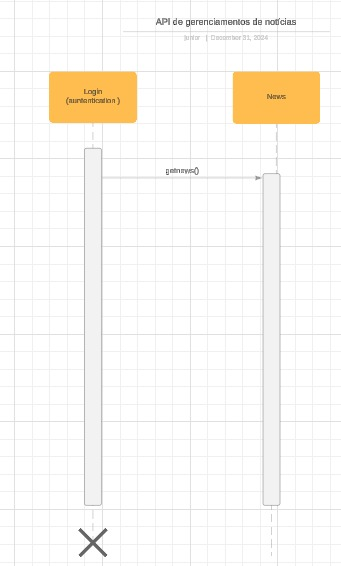
\includegraphics[width=0.5\linewidth]{imagens/sequencia diagrama.jpeg}
    \caption*{\textbf{Fonte:} Elaborado pelo autor usando Lucidchart.}
    \label{fig:enter-label}
\end{figure}

\subsubsection{Diagrama de Classes}

O diagrama de classes representa a estrutura lógica do sistema, identificando as principais entidades e suas relações:
\begin{itemize}
    \item \textbf{Administrador:} É uma subclasse de usuário com permissões adicionais para criar, editar e excluir notícias.
    \item \textbf{Usuário:} Entidade principal que representa qualquer pessoa autenticada no sistema, com funcionalidades como listar notícias e interagir (curtir ou descurtir).
    \item \textbf{Login:} Responsável pela entrada de usuários, vinculada à entidade de usuário.
    \item \textbf{Notícia:} Armazena informações sobre o conteúdo, autor, data de publicação, curtidas e outras propriedades relacionadas às notícias.
\end{itemize}
O diagrama também destaca a herança entre as classes \texttt{Administrador} e \texttt{Usuário}, indicando que administradores possuem todos os atributos e métodos de usuários, além de funcionalidades adicionais.


\begin{figure} [H]
    \centering
    \caption{Diagrama de Classe}
    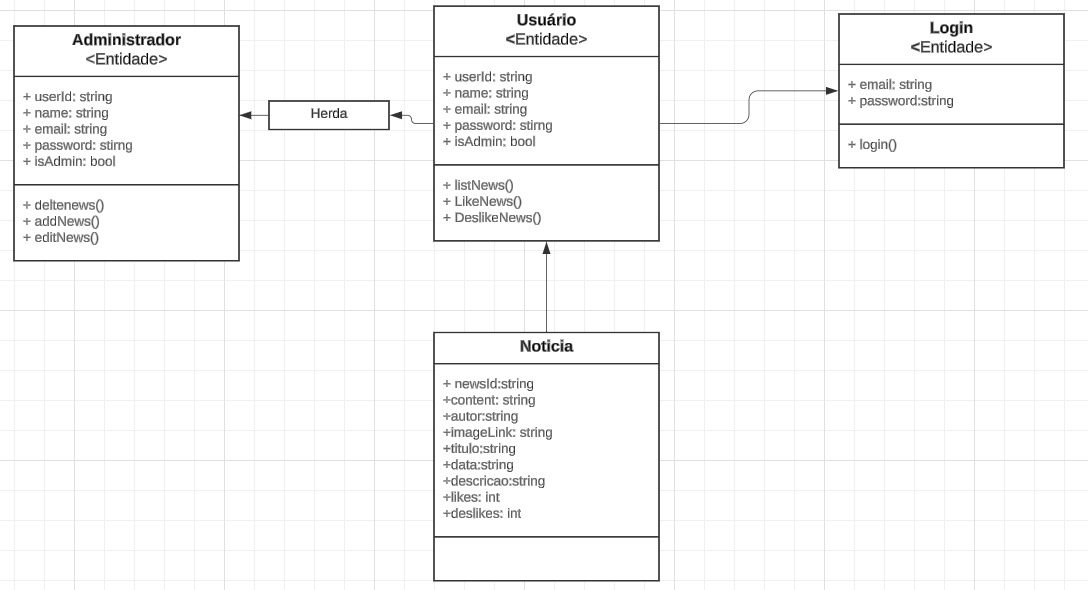
\includegraphics[width=0.5\linewidth]{imagens/diagram de objeto.jpeg}
    \caption*{\textbf{Fonte:} Elaborado pelo autor usando Lucidchart.}
    \label{fig:enter-label}
\end{figure}

\subsubsection{Diagrama de Caso de Uso}

O diagrama de caso de uso detalha as funcionalidades disponíveis para os diferentes atores do sistema:
\begin{itemize}
    \item \textbf{Usuário:} Pode listar notícias e interagir com elas (curtir ou descurtir).
    \item \textbf{Administrador:} Além das funcionalidades do usuário, pode criar, editar e excluir notícias. Essas ações estão associadas às permissões administrativas.
    \item \textbf{Sistema:} O sistema organiza essas interações para garantir que cada ator execute apenas as ações permitidas.
\end{itemize}
Este diagrama enfatiza a separação clara de responsabilidades entre os atores e a funcionalidade do sistema.



\begin{figure} [H]
    \centering
    \caption{Diagrama de Caso de Uso}
    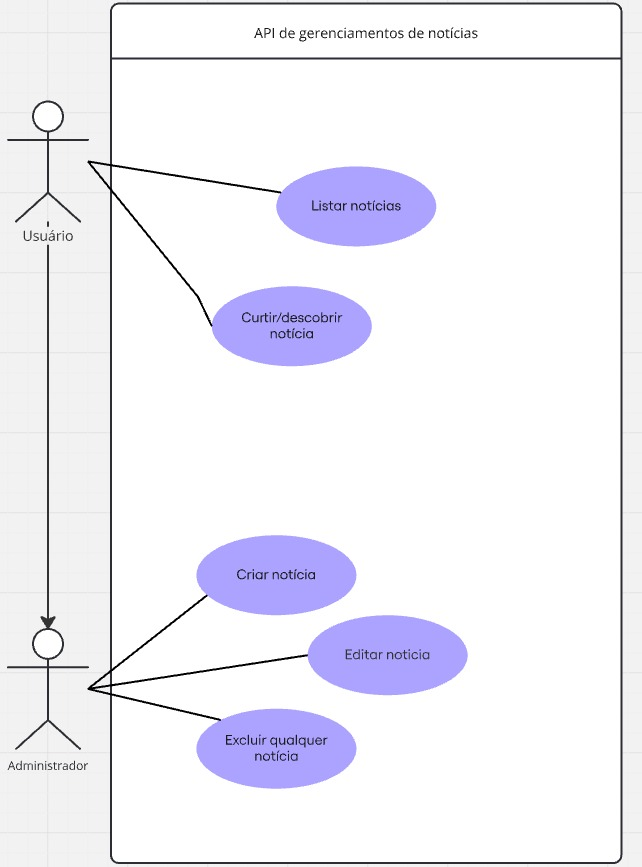
\includegraphics[width=0.5\linewidth]{imagens/diagram de caso de uso.jpeg}
    \caption*{\textbf{Fonte:} Elaborado pelo autor usando Miro.}
    \label{fig:enter-label}
\end{figure}



\chapter{Conceitos Funcionais}

Neste capítulo, exploramos os principais conceitos que fundamentam o paradigma de programação funcional. Esses conceitos são essenciais para compreender a abordagem funcional em comparação com paradigmas imperativos, como a programação orientada a objetos. Além de uma explicação teórica, são apresentados exemplos práticos em Clojure, uma linguagem funcional que foi utilizada no desenvolvimento deste trabalho.


\subsection{Imutabilidade}

A imutabilidade é um dos pilares da programação funcional (\citeonline{Higginbotham15}). Objetos imutáveis não podem ser alterados após sua criação. Isso reduz efeitos colaterais, melhora a previsibilidade do código e facilita a depuração. aplicar os conceitos em programas orientados objetos pode ser de grande benefício para esse software em questão.

\begin{tcolorbox}[colback=gray!5!white, colframe=gray!75!black, title={Quadro 7 - Imutabilidade}]
\begin{lstlisting}[language=Lisp]

(def lista-original [1 2 3])
(def lista-nova (conj lista-original 4)) ; Adiciona 4 sem modificar a lista original

;; Resultado:
;; lista-original => [1 2 3]
;; lista-nova => [1 2 3 4]

\end{lstlisting}
\caption{Exemplo de imutabilidade na linguagem Clojure.}
\end{tcolorbox}

A imutabilidade facilita o desenvolvimento de sistemas concorrentes, pois elimina a necessidade de controle de acesso simultâneo a dados compartilhados. Mas por que devemos nos preocupar com a imutabilidade em nossos códigos?
Os fabricantes de chips já atingiram os limites físicos da miniaturização de transistores. Como consequência, os "ticks" de clock das CPUs não aumentaram desde 2004. A estratégia atual para melhorar o desempenho está no uso de processadores multicore. No entanto, rotinas que compartilham estado mutável não podem ser executadas paralelamente em múltiplos núcleos de forma segura, enquanto a imutabilidade garante a segurança entre threads.
Além disso, a reatribuição de variáveis pode complicar a depuração de erros. Para reproduzir um bug complexo, é necessário compreender a sequência de cálculos que levou ao problema. Alterar variáveis durante a execução pode descartar essa sequência, tornando a análise de falhas mais difícil.


\subsubsection*{Como evitar mutações?}
Sempre que precisar modelar uma mudança de estado, você passa o valor anterior para uma função que retorna um novo valor. Não mude o valor antigo, apenas retorne um novo.

A API desenvolvida neste trabalho apresenta um exemplo simplificado para salvar notícias no banco de dados:

\begin{tcolorbox}[colback=gray!5!white, colframe=gray!75!black, title={Quadro 8 - Integração com Supabase}]
\begin{lstlisting}[language=Lisp]
(let [url "https://supabase.co/rest/v1/noticias"
      headers {"Authorization" (str "Bearer " token)
               "Content-Type" "application/json"}
  (client/post url {:headers headers :form-params body :as :json}))
\end{lstlisting}
\caption{Exemplo simplificado de salvamento de notícias no banco Supabase.}
\end{tcolorbox}

O mapa body é criado como uma nova estrutura de dados para cada notícia iterada, sem alterar o objeto original (noticia). Essa prática evita mudanças inesperadas no estado dos dados, garantindo maior previsibilidade e segurança no sistema. Objetos, sendo referências, podem gerar situações de estados pouco claros se suas propriedades forem alteradas. Ao evitar mudanças nos objetos após sua construção, conseguimos um código mais simples de entender, testar e depurar. Essa abordagem reflete os benefícios da imutabilidade, como a eliminação de efeitos colaterais e a simplificação do fluxo de dados. Além disso, ela promove um design alinhado aos princípios funcionais, especialmente em operações críticas, como interações com bancos de dados externos, resultando em sistemas mais robustos e previsíveis.

\subsection{lazy Evaluation}

A avaliação preguiçosa, ou lazy evaluation, é um conceito importante na programação funcional. Esse paradigma permite que valores sejam calculados apenas quando realmente necessários, diferentemente da avaliação estrita, onde todas as expressões são resolvidas imediatamente. Essa técnica otimiza o uso de recursos, permitindo o processamento eficiente de grandes coleções de dados ou até mesmo de coleções infinitas.

No contexto da API desenvolvida em Clojure, a avaliação preguiçosa é ilustrada pela manipulação de uma sequência infinita com o uso da função `range` combinada com `take`. Isso garante que apenas os valores estritamente necessários sejam calculados, otimizando o uso de memória e processamento. 

\begin{tcolorbox}[colback=gray!5!white, colframe=gray!75!black, title={Quadro 9 - Exemplo de Lazy Evaluation em Clojure}]
\begin{lstlisting}[language=Lisp]
(def numeros (range)) ; Cria uma sequência infinita

(take 5 numeros) ; Extrai os primeiros 5 números: [0 1 2 3 4]
\end{lstlisting}
\caption{Uso de lazy evaluation para manipulação de uma sequência infinita.}
\end{tcolorbox}

A implementação em Clojure também pode ser usada para listar notícias de forma paginada, retornando apenas o número de itens solicitados pela requisição:

\begin{tcolorbox}[colback=gray!5!white, colframe=gray!75!black, title={Quadro 10 - Exemplo de Paginação com Lazy Evaluation em Clojure}]
\begin{lstlisting}[language=Lisp]
(defn listar-noticias
  "Lista as notícias do banco de forma paginada"
  [limite]
  (let [url "https://supabase.co/rest/v1/noticias"
        headers {"Authorization" (str "Bearer " (get-supabase-token))
                 "Content-Type" "application/json"}
        noticias (:body (client/get url {:headers headers :as :json}))]
    (take limite noticias))) ; Retorna apenas as primeiras 'limite' notícias
\end{lstlisting}
\caption{Implementação de paginação utilizando lazy evaluation em Clojure.}
\end{tcolorbox}

Por outro lado, a implementação em Java, utilizando o paradigma orientado a objetos, não apresenta suporte nativo à lazy evaluation. No exemplo abaixo, todas as notícias são recuperadas do banco de dados em uma única requisição, e qualquer tipo de filtragem ou paginação deve ser implementada explicitamente, gerando maior uso de memória para grandes volumes de dados:

\begin{tcolorbox}[colback=gray!5!white, colframe=gray!75!black, title={Quadro 11 - Paginação em Java sem Lazy Evaluation}]
\begin{lstlisting}[language=Java]
// Endpoint no controlador
@GetMapping
public ResponseEntity<?> getAllNews() {
    try {
        List<News> news = service.getAllNews(); 
        return ResponseEntity.ok(news); 
    }
}

// Service responsável pela request
public List<News> getAllNews() {
    String url = supabaseUrl + "/noticias";
    HttpHeaders headers = createHeaders(supabaseApiKey); 
    ResponseEntity<List<News>> response = restTemplate.
    );
    return response.getBody(); 
}
\end{lstlisting}
\caption{Exemplo simplificado de paginação em Java sem suporte nativo à lazy evaluation.}
\end{tcolorbox}


\subsubsection*{Análise Comparativa}

A principal diferença entre as implementações em Clojure e Java está no suporte ao conceito de avaliação preguiçosa. No Clojure, a função `take` permite que apenas os elementos necessários sejam processados, garantindo economia de memória e eficiência ao lidar com grandes conjuntos de dados ou sequências infinitas. Essa abordagem está alinhada aos princípios da programação funcional, eliminando efeitos colaterais e facilitando a manutenção do código. Já na implementação em Java, todo o conjunto de dados é recuperado do banco de dados em uma única operação, carregando todas as notícias na memória antes que qualquer filtragem ou paginação seja aplicada. Isso aumenta o uso de recursos e a complexidade de escalabilidade do sistema, especialmente em cenários de alto volume de dados. Embora o paradigma orientado a objetos ofereça maior familiaridade para muitos desenvolvedores, ele exige um esforço adicional para simular comportamentos semelhantes ao lazy evaluation.

Assim, observa-se que a abordagem funcional é mais eficiente e previsível em termos de manipulação de dados, enquanto a implementação orientada a objetos, embora robusta, não oferece suporte nativo a recursos como a avaliação preguiçosa.

\subsection{Recursão}

A recursão é um dos conceitos fundamentais da programação funcional. Ela permite que uma função chame a si mesma para resolver um problema, quebrando-o em partes menores até atingir uma condição base. Diferentemente de laços tradicionais (como for ou while), a recursão se alinha ao paradigma funcional por evitar estados mutáveis e depender apenas de funções puras.

Em linguagens funcionais como Clojure, a recursão é amplamente utilizada para iterar sobre coleções, processar dados ou executar cálculos matemáticos. Além disso, muitas linguagens funcionais otimizam recursão em cauda (*tail recursion*), o que evita o estouro de pilha em chamadas recursivas profundas.

A recursão apresenta diversos benefícios na programação funcional, como a ausência de estados mutáveis. Isso resulta em código mais seguro, previsível e fácil de depurar. Além disso, a recursão promove clareza e concisão, eliminando a necessidade de estruturas de controle complexas, como laços tradicionais.

\begin{tcolorbox}[colback=gray!5!white, colframe=gray!75!black, title={Quadro 12 - Exemplo de Recursão em Clojure}]
\begin{lstlisting}[language=Lisp]
(defn soma-curtidas [noticias]
  (if (empty? noticias)
    0
    (+ (:likes (first noticias)) (soma-curtidas (rest noticias)))))

;; Exemplo de uso:
(def noticias [{:title "Notícia 1" :likes 10}
               {:title "Notícia 2" :likes 20}
               {:title "Notícia 3" :likes 15}])

(soma-curtidas noticias) ; Resultado: 45
\end{lstlisting}
\caption{Exemplo de cálculo recursivo em Clojure para somar as curtidas de uma lista de notícias.}
\end{tcolorbox}

No exemplo acima, a função `soma-curtidas` processa recursivamente cada item da lista de notícias, somando os valores de curtidas até que a lista esteja vazia. Cada chamada recursiva é independente, eliminando estados mutáveis e promovendo previsibilidade.

A seguir, apresentamos uma abordagem equivalente em Java, utilizando o paradigma orientado a objetos. Nesse caso, a soma de curtidas é realizada iterativamente, mantendo estados mutáveis:

\begin{tcolorbox}[colback=gray!5!white, colframe=gray!75!black, title={Quadro 13 - Exemplo Iterativo em Java}]
\begin{lstlisting}[language=Java]
public int somaCurtidas(List<News> noticias) {
    int total = 0;
    for (News noticia : noticias) {
        total += noticia.getLikes();
    }
    return total;
}
\end{lstlisting}
\caption{Exemplo de cálculo iterativo em Java para somar curtidas.}
\end{tcolorbox}

\subsubsection*{Análise Comparativa}

A principal diferença entre as abordagens em Clojure e Java está na forma como as operações são realizadas. Em Clojure, a soma das curtidas utiliza recursão, eliminando estados mutáveis e garantindo que cada chamada seja uma função pura. Essa abordagem é mais alinhada aos princípios da programação funcional, como clareza e previsibilidade.

Por outro lado, a implementação em Java utiliza um loop `for`, que depende de um estado mutável (`total`) para armazenar o resultado intermediário. Embora a abordagem seja eficiente e direta, ela está mais sujeita a erros, especialmente em cenários mais complexos, onde estados mutáveis podem levar a comportamentos inesperados.

Ambas as abordagens são funcionais em seus respectivos contextos, mas a recursão em Clojure oferece vantagens em termos de simplicidade, alinhamento ao paradigma funcional e facilidade de manutenção em sistemas maiores.

\subsection{Monoids}

O conceito de monóides, explorado em profundidade no livro Learn You a Haskell for Great Good!, de Miran Lipovača (\citeonline{Lipovaca11}), que é um dos livros estudados para construção deste trabalho, apresenta-se como uma poderosa abstração matemática que desempenha um papel fundamental na programação funcional. Um monóide é uma estrutura algébrica que consiste em um conjunto, uma operação binária e um elemento neutro. Na prática, isso significa que um monóide deve satisfazer duas propriedades principais: associatividade e a existência de um elemento neutro.
A associatividade garante que a ordem em que as operações são realizadas não afeta o resultado. Já o elemento neutro assegura que, ao combinar qualquer valor com ele, o valor original permaneça inalterado. Em Haskell, os monóides são definidos por meio da typeclass Monoid, que exige a implementação das operações mempty (o elemento neutro) e mappend (a operação de combinação), além de oferecer uma função mconcat para combinar listas de elementos.


\begin{tcolorbox}[colback=gray!5!white, colframe=gray!75!black, title={Quadro 14 - Exemplo de Definição e Uso de Monóides em Haskell}]
\begin{lstlisting}[language=Haskell]
-- Definindo um monóide para números inteiros com adição
instance Monoid Integer where
    mempty = 0               -- Elemento neutro para adição
    mappend = (+)            -- Operação binária: soma

-- Uso prático
mconcat [1, 2, 3, 4]         -- Resultado: 10
\end{lstlisting}
\caption{Definição de um monóide para números inteiros e sua utilização prática em Haskell.}
\end{tcolorbox}

Neste exemplo, números inteiros formam um monóide em que o elemento neutro é 0, pois somar qualquer número a 0 não altera o número, e a operação binária é a soma. 

O uso de monóides simplifica a construção de funções genéricas e abstrações elegantes. Por exemplo, listas em Haskell formam um monóide, onde a operação binária é a concatenação e o elemento neutro é a lista vazia. Da mesma forma, tipos numéricos podem ser monóides sob adição (com o zero como elemento neutro) ou multiplicação (com o um como elemento neutro).

Essa estrutura é amplamente utilizada em contextos como agregação de dados, combinação de resultados e processamento paralelo, onde a associatividade e o elemento neutro permitem que cálculos sejam divididos e reagrupados de forma eficiente.

A aplicação dos monóides transcende a matemática pura e fornece ferramentas práticas para resolver problemas complexos com código conciso, modular e de fácil manutenção. Assim, compreender e aplicar o conceito de monóides é essencial para aproveitar ao máximo o poder da programação funcional.


\chapter{O futuro da programação Funcional}

\subsection{Case Nubank}

Um dos casos mais interessantes do uso da programação funcional é o da Nubank. A Nubank é uma startup brasileira pioneira no segmento de serviços financeiros, atuando como operadora de cartões de crédito e fintech. Fundada em 6 de maio de 2013 e sediada em São Paulo, a empresa conta atualmente com mais de 10 mil colaboradores e é amplamente reconhecida por ter revolucionado não apenas o mercado financeiro, mas também a indústria de software no Brasil. A Nubank foi uma das pioneiras na adoção do paradigma funcional em grande escala, utilizando a linguagem de programação Clojure para reduzir a complexidade dos seus serviços.

No artigo “O que é programação funcional e como usamos esta tecnologia no Nubank?”, publicado no blog oficial da empresa, Bruno Rodrigues, Senior Engineering Manager na Nubank, explica: 

\begin{quote}
 "Naquele momento, o paradigma funcional parecia ser a melhor opção para os desafios que teríamos que enfrentar. Por causa disso, acabamos adotando o Clojure como a linguagem principal para os nossos serviços e o Datomic como nosso banco de dados." - (\citeonline{Rodrigues2022})
\end{quote}
 
 Essa escolha estratégica permitiu à Nubank criar um ecossistema robusto e escalável, utilizando as vantagens da imutabilidade e da composição de funções características da programação funcional.

Em 2020, a Nubank adquiriu a Cognitect, uma empresa norte-americana de consultoria e desenvolvimento de software sediada em Durham, Carolina do Norte, conhecida por ser a casa da renomada Universidade de Duke. A Cognitect trouxe para a Nubank um time de especialistas de alto nível, incluindo Rich Hickey, criador da linguagem Clojure e designer do banco de dados Datomic. Essa aquisição não só reforçou a expertise técnica da Nubank, mas também consolidou sua posição como referência global na aplicação de paradigmas funcionais em sistemas financeiros.

\subsection{Desafio em ensino em universidades}

Embora a programação funcional seja um tema extremamente interessante e com grande potencial para contribuir na formação de profissionais da área de TI, ainda é pouco abordada nas universidades brasileiras. Em uma pesquisa realizada sobre a grade curricular de cursos em instituições públicas e privadas no Brasil, constatou-se que, na maioria dos casos, não há disciplinas específicas que abordem o paradigma funcional.
Quando o tema é incluído nos currículos, geralmente está presente em instituições públicas, como a UFPR, UNIFEI, FATEC e USP, que oferecem disciplinas regulares e optativas relacionadas, como “Introdução ao Cálculo Lambda”. Apesar disso, essas iniciativas ainda são exceções e não refletem uma abordagem sistemática para o ensino do paradigma funcional no contexto acadêmico.
A escassez de disciplinas dedicadas ao tema pode ser atribuída a diversos fatores, como a falta de docentes especializados na área, o foco predominante em paradigmas imperativos e orientados a objetos, e a percepção de que a programação funcional é mais complexa, sendo algo de mais “baixo nível”. Entretanto, essa visão ignora o fato de que a programação funcional não apenas facilita a construção de sistemas mais robustos e escaláveis, mas também proporciona um entendimento mais profundo sobre a teoria da computação e a abstração algébrica, competências cada vez mais valorizadas na indústria de tecnologia. Assim, com junto com o crescimento do uso linguagens funcionais no mercado de trabalho brasileiro e estrangeiro, acredito que irá ser tornar mais encontrar cadeira sobre o assunto em insituiçẽs de ensino, a partir de uma maior demanda do mercado. 


\subsection{Tendências e Futuro da Programação Funcional}

A programação funcional tem ganhado cada vez mais relevância no cenário tecnológico, acompanhando a crescente demanda por sistemas mais escaláveis, seguros e de fácil manutenção. Embora historicamente tenha sido considerada um paradigma acadêmico, ela está sendo amplamente adotada na indústria devido às suas vantagens intrínsecas, como a imutabilidade, funções puras e composição. Esses conceitos são particularmente valiosos em um contexto de computação distribuída, big data e inteligência artificial.
Uma das tendências mais notáveis é a integração de características funcionais em linguagens populares orientadas a objetos, como Java, C# e Python. Funcionalidades como lambdas, funções de ordem superior e imutabilidade têm se tornado padrões, permitindo que desenvolvedores combinem os benefícios da programação funcional com paradigmas imperativos.
Outra tendência importante é o uso de linguagens funcionalmente puras, como Haskell, Clojure, Scala e Elixir, em aplicações de alto desempenho e sistemas críticos. Empresas como Nubank, Twitter e WhatsApp já demonstraram o impacto positivo dessas linguagens na construção de soluções confiáveis e eficientes. Um ponto interessante a ser destacado é a atratividade financeira das linguagens funcionais. Segundo uma pesquisa realizada pelo canal Código Fonte no YouTube, que é focado em assuntos relacionados à tecnologia e conta com milhões de seguidores, as linguagens funcionais apresentam uma média salarial de aproximadamente 16 mil reais no Brasil (\citeonline{CodigoFonte2024}). Essa pesquisa, conduzida anualmente com profissionais da área, aborda diversos temas, incluindo a remuneração média por linguagem, e os dados indicam que a alta remuneração é um dos fatores que atraem novos profissionais para esse paradigma. Além disso, a popularidade de bibliotecas e frameworks funcionais em linguagens mainstream, como React (JavaScript) e Spark (Python/Scala), reflete a influência crescente do paradigma funcional no desenvolvimento moderno. O futuro da programação funcional parece promissor, especialmente em áreas como computação paralela e concorrente, onde a imutabilidade e a ausência de estados mutáveis tornam esse paradigma ideal para sistemas que exigem processamento paralelo seguro e eficiente. Além disso, na inteligência artificial e no aprendizado de máquina, os modelos matemáticos e cálculos algébricos, que são pilares da programação funcional, encontram aplicação direta no treinamento e na análise de algoritmos. Por fim, no desenvolvimento de software escalável, a adoção de paradigmas funcionais têm contribuído significativamente para resolver problemas de escalabilidade em sistemas distribuídos e em aplicações web de grande porte.
No entanto, para que a programação funcional atinja todo o seu potencial, será necessário superar desafios relacionados ao ensino e à aceitação no mercado. Isso inclui a necessidade de uma maior capacitação de desenvolvedores e a adaptação de ferramentas para facilitar sua adoção em projetos do dia a dia.
Com a evolução contínua da tecnologia e a crescente complexidade dos sistemas computacionais, a programação funcional se consolida como uma ferramenta indispensável para enfrentar os desafios do futuro, oferecendo soluções elegantes, eficientes e sustentáveis.



%=======================================================================
% Exemplos de Citações e Referências Bibliográficas
%=======================================================================
\chapter{RESULTADOS E DISCUSSÃO}

Este capítulo apresenta os resultados obtidos durante o desenvolvimento do trabalho e discute suas implicações. Nele, são comparados os paradigmas de programação funcional e orientada a objetos, tomando como referência as duas APIs desenvolvidas: uma em Java, estruturada no paradigma orientado a objetos, e outra em Clojure, fundamentada no paradigma funcional. Além disso, os resultados são discutidos à luz da literatura revisada, destacando como cada abordagem impacta a escalabilidade, manutenção e implementação de sistemas.

\section{Comparação entre as APIs Desenvolvidas}

Durante o desenvolvimento das APIs, foram identificadas diferenças significativas nos paradigmas utilizados. Essas diferenças influenciaram diretamente a estruturação do código, a complexidade do sistema e os desafios de manutenção. Para ilustrar essas diferenças, são apresentadas trechos relevantes de código para análise comparativa.

\subsection{Estrutura do Código}

O pesquisador britânico Simon Peyton Jones, um dos principais desenvolvedores da linguagem funcional Haskell e autor de diversos artigos sobre programação funcional e otimização de compiladores, destaca que "a imutabilidade da programação funcional elimina a necessidade de bloqueios e sincronização complexa em ambientes concorrentes" (Peyton, 23).
Essa característica foi evidente na estrutura do código em Clojure, que demonstrou ser mais concisa, com um foco maior em funções puras e imutabilidade. A API funcional foi construída utilizando um modelo declarativo, no qual as operações são descritas em termos do que deve ser feito, em vez de como fazê-lo.
Essa abordagem é exemplificada no Quadro 15, que apresenta a implementação de uma listagem de notícias em Clojure, minimizando o uso de estados mutáveis e reduzindo efeitos colaterais.



\begin{center}
    \textbf{Quadro 15 - Listagem de Notícias em Clojure}
\end{center}

\begin{tcolorbox}[colback=gray!5!white, colframe=gray!75!black, title=]
\begin{lstlisting}[language=Lisp]
(defn listar-noticias [limite]
  (let [url "https://supabase.co/rest/v1/noticias"
        noticias (:body (client/get url {:headers headers :as :json}))]
    (take limite noticias)))
\end{lstlisting}
\caption{Exemplo de listagem de notícias utilizando lazy evaluation em Clojure.}
\end{tcolorbox}

\begin{center}
    \textit{Fonte: Elaborado pelo autor, 2024} 
\end{center}

Em contrapartida, a implementação em Java, utilizando uma abordagem imperativa, é ilustrada no Quadro 16, evidenciando a necessidade de maior controle manual de estados e tratamento explícito de exceções. Essa característica reflete um dos desafios apontados por (Sandi, 2013), que destaca que "a complexidade desnecessária na programação orientada a objetos pode ser minimizada por meio de boas práticas de design". A dependência de estados mutáveis e a necessidade de gerenciar manualmente exceções podem aumentar a verbosidade e a dificuldade de manutenção do código, torna-se essencial a adoção de padrões que reduzam essa complexidade.

\begin{center}
    \textbf{Quadro 16 - Listagem de Notícias em Java}
\end{center}

\begin{tcolorbox}[colback=gray!5!white, colframe=gray!75!black, title=]
\begin{lstlisting}[language=Java]
public List<News> listarNoticias(int limite) {
    String url = supabaseUrl + "/noticias";
    HttpHeaders headers = new HttpHeaders();
    headers.set("Authorization", "Bearer " + supabaseApiKey);
    ResponseEntity<List<News>> response = restTemplate.exchange(
    );
    return response.getBody().stream().limit(limite).collect(Collectors.toList());
}
\end{lstlisting}
\end{tcolorbox}
\begin{center}
    \textit{Fonte: Elaborado pelo autor, 2024} 
\end{center}

\subsection{Manutenibilidade e Leitura do Código}

Os resultados mostram que o código em Clojure é mais legível e modular devido ao uso de funções puras e à imutabilidade. Esses fatores simplificam a adição de novas funcionalidades, reduzindo a necessidade de revisar partes já implementadas. Na API em Java, a dependência de estados mutáveis e exceções tornou algumas partes do código mais verbosas e difíceis de entender.

Esses achados estão alinhados com os estudos de Lipovača (Lipovaca, 11), que destaca como a imutabilidade reduz a complexidade em sistemas concorrentes e de grande escala.

\subsection{Desempenho e Escalabilidade}

Nos testes realizados, ambas as APIs apresentaram tempos de resposta semelhantes em operações básicas. No entanto, em cenários que envolviam execução paralela, a API funcional apresentou maior eficiência devido à imutabilidade, que elimina a necessidade de mecanismos complexos de controle de estado, como locks. 

\subsection{Integração com a Literatura}

Os resultados observados reforçam as vantagens descritas na literatura sobre a programação funcional, como maior previsibilidade e facilidade de manutenção. No entanto, os desafios apontados também são corroborados por autores como Hughes (Hughes, 90), que enfatiza a curva de aprendizado como uma barreira para adoção do paradigma funcional.

\subsection{Discussão}

A comparação entre as APIs mostra que o paradigma funcional oferece vantagens significativas em sistemas complexos e escaláveis, especialmente em cenários de concorrência, onde a imutabilidade e a ausência de efeitos colaterais simplificam o controle do estado.

Por outro lado, a programação orientada a objetos (POO) continua sendo amplamente utilizada devido à sua familiaridade e suporte da indústria, além da vasta disponibilidade de ferramentas e frameworks que facilitam sua adoção. No entanto, a necessidade de lidar com estados mutáveis e exceções pode aumentar consideravelmente a complexidade de sistemas maiores, dificultando a manutenção a longo prazo.
Martin Fowler (1999) argumenta que "a refatoração permite que sistemas escritos em paradigmas diferentes adotem melhores práticas para aumentar a legibilidade e reduzir a complexidade". Isso sugere que, independentemente do paradigma escolhido, a qualidade do design e a clareza do código são fatores determinantes para a manutenção e escalabilidade do software. No contexto da POO, técnicas de refatoração ajudam a reduzir a rigidez estrutural do código, enquanto na programação funcional, a modularidade inerente tende a favorecer soluções mais expressivas e enxutas.

A adoção de padrões de projeto é frequentemente apontada como um meio de melhorar a reutilização e organização do código em sistemas orientados a objetos "A utilização de padrões de projeto na programação orientada a objetos facilita a manutenção do código e melhora sua escalabilidade" (Gamma et al., 1995). No entanto, apesar de sua importância, a aplicação rigorosa desses padrões pode levar a um aumento excessivo da complexidade estrutural. Em projetos muito grandes, a necessidade de seguir múltiplos padrões simultaneamente pode tornar o código difícil de entender e modificar, resultando em uma arquitetura excessivamente fragmentada e burocrática. Isso cria um paradoxo: embora os padrões tenham sido desenvolvidos para simplificar o design de software, sua implementação em larga escala pode acabar tornando o sistema ainda mais difícil de gerenciar.
Os resultados obtidos também mostram que conceitos funcionais, como imutabilidade e composição de funções, podem ser incorporados em linguagens não funcionais para melhorar a qualidade do código. Conforme destacado por (Fowler, 1999), boas práticas de design independem do paradigma adotado. Por exemplo, o uso de objetos imutáveis e funções puras pode ser aplicado em linguagens como Java e Python, proporcionando maior previsibilidade e reduzindo o acoplamento do código, mesmo fora do contexto de uma linguagem funcional.

\subsection{Limitações do Estudo}

Embora os resultados demonstrem as vantagens do paradigma funcional, o estudo teve algumas limitações:
\begin{itemize}
    \item O número de cenários testados foi limitado, o que pode restringir a generalização dos resultados.
    \item A comparação focou em APIs relativamente simples, o que pode não refletir desafios de sistemas de grande escala.
    \item A análise de desempenho foi restrita a casos específicos, sem considerar cenários extremos.
\end{itemize}

Futuros estudos podem explorar casos mais complexos, envolvendo cargas de trabalho maiores e integrações mais robustas com bibliotecas e ferramentas de mercado.




\chapter{CONSIDERAÇÕES FINAIS}

O presente trabalho buscou explorar o paradigma funcional, um modelo de programação que, apesar de não ser novo, tem ganhado cada vez mais espaço em um cenário tecnológico em constante evolução. Partindo de uma análise histórica e conceitual, até aplicações práticas no mercado, como o uso de linguagens funcionais por empresas como a Nubank, foi possível compreender como a programação funcional pode contribuir significativamente para o desenvolvimento de software mais eficiente, seguro e escalável.

Através do desenvolvimento de duas APIs no âmbito deste trabalho – uma em Java, utilizando o paradigma orientado a objetos, e outra em Clojure, baseada no paradigma funcional – foi possível realizar uma comparação prática entre os dois modelos. Essa abordagem demonstrou, na prática, os benefícios da imutabilidade, funções puras e composição, pilares fundamentais da programação funcional. Além disso, permitiu verificar como a escolha de um paradigma pode impactar diretamente a simplicidade, manutenção e robustez do software.
No decorrer do estudo, também foi destacado o papel da programação funcional no mercado atual, onde a crescente adoção de linguagens como Haskell, Elixir, e Clojure reflete uma demanda por soluções que promovam escalabilidade e confiabilidade. Contudo, a análise revelou desafios, especialmente no âmbito acadêmico, onde o paradigma funcional ainda é pouco abordado nos currículos das universidades brasileiras. Este cenário reforça a necessidade de ampliar o ensino e a divulgação dessa abordagem, preparando melhor os profissionais de TI para atender às demandas da indústria.
Dentre as principais contribuições deste trabalho, destaca-se a contextualização teórica e prática da programação funcional, oferecendo uma base para que outros desenvolvedores e pesquisadores explorem o tema. A experiência prática desenvolvida durante o projeto também demonstrou que paradigmas como o funcional não são apenas teoricamente interessantes, mas também aplicáveis a problemas reais.

Por fim, este estudo reforça a importância de pensar funcionalmente, não apenas como um conceito técnico, mas como uma filosofia de desenvolvimento. É possível implementar os princípios da programação funcional em linguagens que não são puramente funcionais, como JavaScript e Python, aproveitando características como imutabilidade e funções puras para tornar o código mais seguro, previsível e modular. Essa abordagem contribui diretamente para o desenvolvimento de sistemas mais robustos e alinhados às demandas do mercado atual.
O trabalho realizado também abre espaço para pesquisas futuras, como a aplicação do paradigma funcional em áreas emergentes, incluindo inteligência artificial e computação paralela, onde a imutabilidade e a ausência de estados mutáveis podem resolver problemas de concorrência com maior eficiência. Além disso, destaca-se a importância de explorar mais profundamente os desafios de sua adoção no ensino acadêmico e na indústria, promovendo a disseminação desse paradigma e preparando os profissionais para utilizá-lo de forma eficaz em projetos reais.
\cite{Hughes90}, \cite{Lipovaca11}, \cite{Kay93}, \cite{Hickey2020}, \cite{Church1936}, \cite{Computerphile2016}, \cite{Higginbotham15}, \cite{Rodrigues2022}, \cite{Codigofonte2024}, \cite{Guedes2020}, \cite{Gamma1995}, \cite{Fowler1999}, \cite{PeytonJones2003}, \cite{Sestoft1997}, \cite{Booch2007}, \cite{Metz2013}




%=======================================================================
% Referências
%=======================================================================
% Descomentar a linha abaixo quando inserir alguma referência bibliográfica
%\bibliography{exemplo}

%=======================================================================
% Exemplo de Apêndice
% O Apêndice é utilizado para apresentar material complementar elaborado
% pelo próprio autor.  Deve seguir as mesmas regras de formatação do
% corpo principal do documento.
%=======================================================================
% \appendix
% \chapter{Informações Complementares}

% Escreva aqui.

%=======================================================================
% Exemplo de Anexo
% O Anexo é utilizado para a ``inclusão de materiais não elaborados pelo
% próprio autor, como cópias de artigos, manuais, folders, balancetes, etc.
% e não precisam estar em conformidade com o modelo''.
%=======================================================================
% \annex
% \chapter{Artigos Publicados}

\bibliography{exemplo}


\appendix
\chapter{Apêndice B}

Este apêndice apresenta os links para os repositórios GitHub das APIs desenvolvidas neste trabalho, permitindo acesso ao código-fonte e à documentação.

\section*{API em Java}
O repositório da API desenvolvida em Java pode ser acessado no seguinte link:
\begin{itemize}
    \item \url{https://github.com/Juniorbasck/API-for-news-management-java}
\end{itemize}

\section*{API em Clojure}
O repositório da API desenvolvida em Clojure pode ser acessado no seguinte link:
\begin{itemize}
    \item \url{https://github.com/Juniorbasck/API-for-news-management-clojure}
\end{itemize}

Para cada repositório, há um arquivo README que explica o funcionamento das APIs, suas funcionalidades e instruções para execução local. Esses repositórios estão disponíveis publicamente para consulta e testes.


\end{document}
